\documentclass{beamer}
	\title{La mia prima presentazione}
	\author{Antonio Michele Miti}
	\date{20 novembre 2015}

% Packages ---------------------------------------------------------------------------------------------------------------------------
%			Standalone non funziona ancora bene con beamer.
\usepackage[mode=buildnew]{standalone}				%\includestandalone[width=\textwidth]{Pictures/GeometricPicture0}
\usepackage{tikz}
\usepackage{pgfplots}
\pgfplotsset{compat=newest}
\usepackage{amsmath}
%------------------------------------------------------------------------------------------------------------------------------------------------------------



%Common symbols
%Common math symbols
	%Number fields
		\newcommand{\Real}{\mathbb{R}}
		\newcommand{\Natural}{\mathbb{N}}
		\newcommand{\Relative}{\mathbb{Z}}
		\newcommand{\Rational}{\mathbb{Q}}
		\newcommand{\Complex}{\mathbb{C}}
	
%equality lingo
	%must be equal
		\newcommand{\mbeq}{\overset{!}{=}} 

% function
	%Domain
		\newcommand{\dom}{\mathrm{dom}}
	%Range
		\newcommand{\ran}{\mathrm{ran}}
	

% Set Theory
	% Power set (insieme delle parti
		\newcommand{\PowerSet}{\mathcal{P}}

%Differential Geometry
	% Atlas
		\newcommand{\Atlas}{\mathcal{A}}
	%support
		\newcommand{\supp}{\textrm{supp}}

	
	
%Category Theory
	%Mor set http://ncatlab.org/nlab/show/morphism
%		\newcommand{\hom}{\textrm{hom}}

%Geometric Lagrangian Mechanics
	% Kinematic Configurations
		\newcommand{\Conf}{\mathtt{C}}
	%Solutions Space
		\newcommand{\Sol}{\mathtt{Sol}}
	%Lagrangian class
		\newcommand{\Lag}{\mathsf{Lag}}
	%Lagrangiana
		\newcommand{\Lagrangian}{\mathcal{L}}
	%Data
		\newcommand{\Data}{\mathsf{Data}}
	%unique solution map
		\newcommand{\SolMap}{\mathbf{s}}
	%Classical Observables
		\newcommand{\Obs}{\mathcal{E}}	
	%Phase Space
		\newcommand{\Phase}{\mathcal{M}}	

		\
		
%Peierls (per non sbagliare più)
		\newcommand{\Pei}{Peierls}
%---------------------------------------------------------------------------------------------------------------------------------------------------------------------

%\usetheme{CambridgeUs}





\begin{document}


%\/\/\/\/\/\/\/\/\/\/\/\/\/\/\/\/\/\/\/\/\/\/\/\/\/\/\/\/\/\/\/\/\/\/\/\/\/\/\/\/\/\/\/\/\/\/\/\/\/\/\/\/\/\/\/\/\/\/\/\/\/\/\/\/\/\/\/\/\/
%				Intro
%\/\/\/\/\/\/\/\/\/\/\/\/\/\/\/\/\/\/\/\/\/\/\/\/\/\/\/\/\/\/\/\/\/\/\/\/\/\/\/\/\/\/\/\/\/\/\/\/\/\/\/\/\/\/\/\/\/\/\/\/\/\/\/\/\/\/\/\/\/
	\begin{frame} %Titolo
		\maketitle
	\end{frame}

%	\section*{Intro}	
	\begin{frame}{Overview}
		(struttura della tesi vs struttura della presentazione)
		\tableofcontents
	\end{frame}

	

%\/\/\/\/\/\/\/\/\/\/\/\/\/\/\/\/\/\/\/\/\/\/\/\/\/\/\/\/\/\/\/\/\/\/\/\/\/\/\/\/\/\/\/\/\/\/\/\/\/\/\/\/\/\/\/\/\/\/\/\/\/\/\/\/\/\/\/\/\/
%				Parte 1 : 	"Foundations of Mechanics"
%\/\/\/\/\/\/\/\/\/\/\/\/\/\/\/\/\/\/\/\/\/\/\/\/\/\/\/\/\/\/\/\/\/\/\/\/\/\/\/\/\/\/\/\/\/\/\/\/\/\/\/\/\/\/\/\/\/\/\/\/\/\/\/\/\/\/\/\/\/		
	\section{Meccanica Geometrica}
		\frame{\sectionpage}
	
		\begin{frame}{Meccanica Geometrica}
  			\begin{columns}[T]
    			\begin{column}{.5\textwidth}		
					\begin{itemize}
						\item L'idea
						\item La scommessa				
					\end{itemize}
    			\end{column}
    		   	\begin{column}{.5\textwidth}
							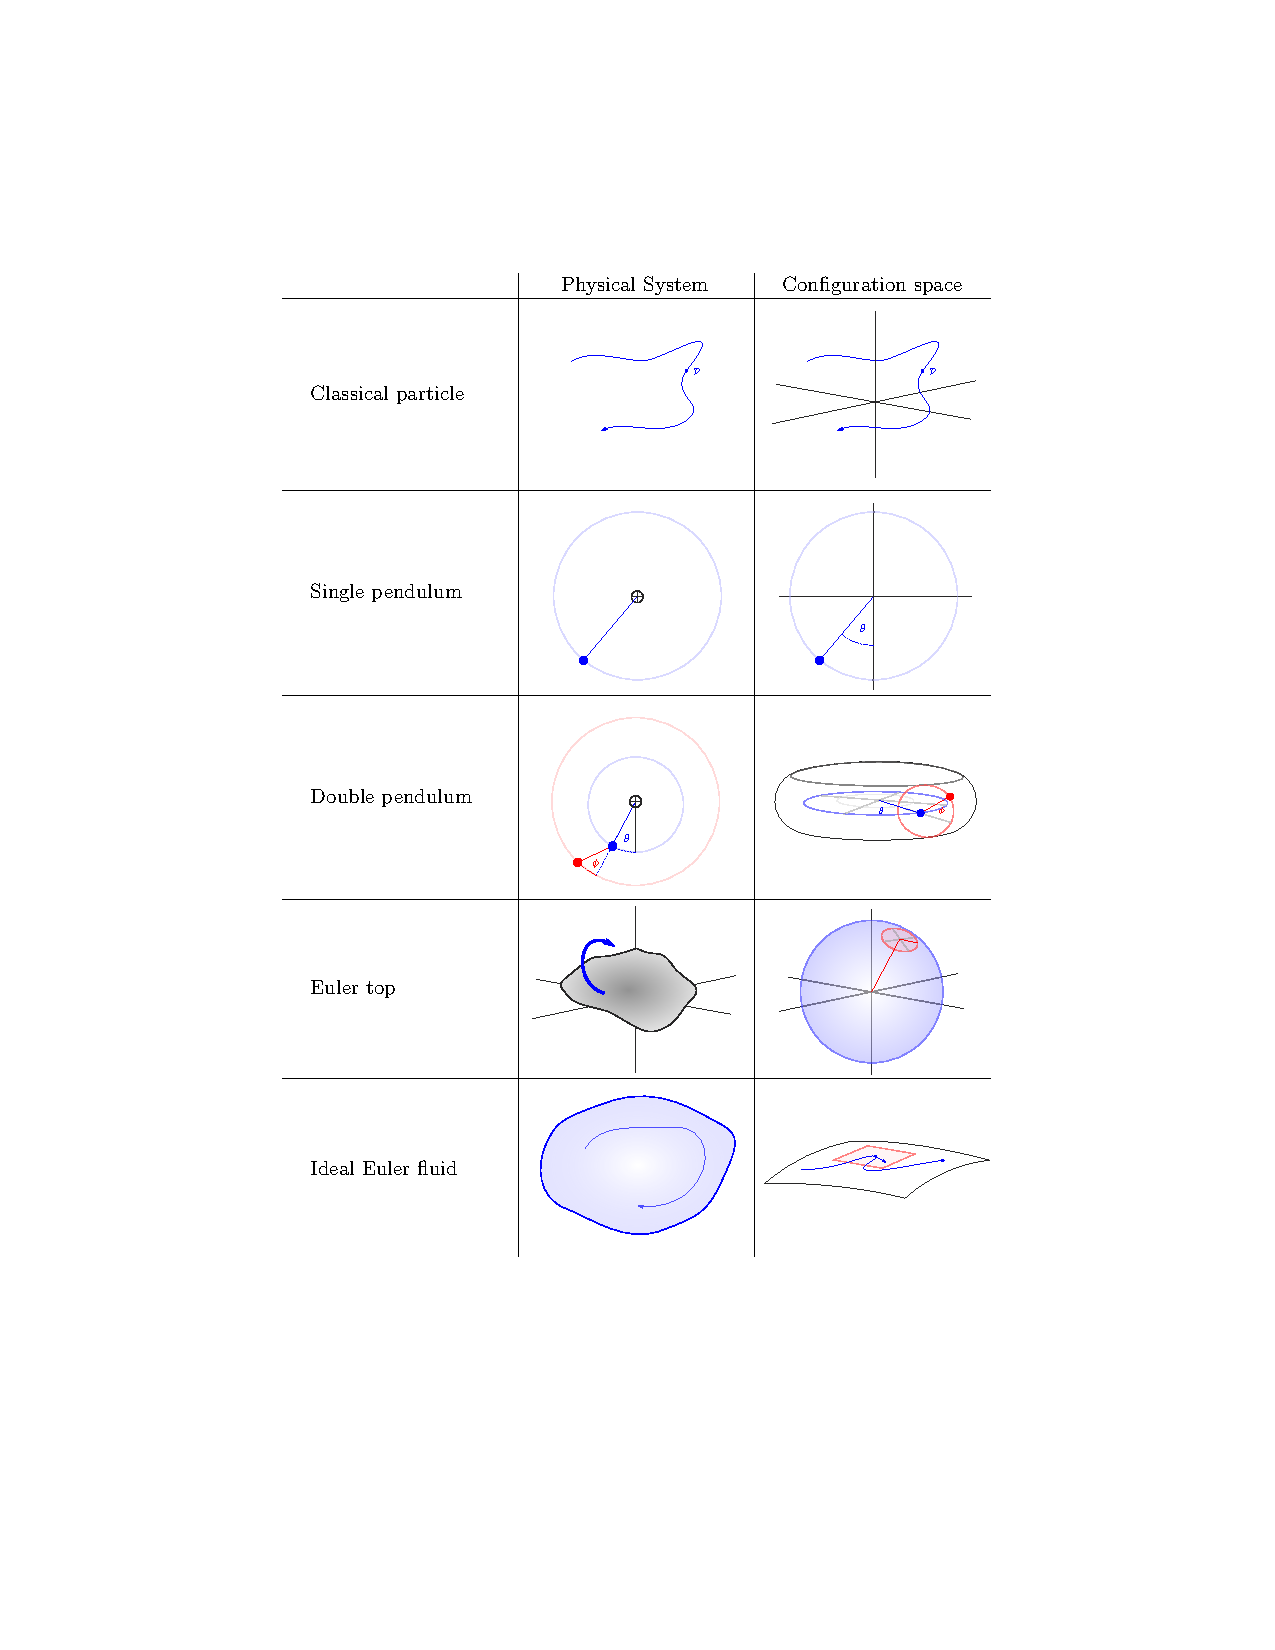
\includegraphics[width=\textwidth]{Presentazione/GeoMec_Crop} 				
    			\end{column}
  			\end{columns}	
	\end{frame}
	
	\begin{frame}
		\frametitle{Formalismo canonico}
  			\begin{columns}[T]
    			\begin{column}{.5\textwidth}
     				\begin{block}{Your textblock}
						% Your text here
						(usual approach) I passi principali per la costruzione del formalismo canonico per teorie con $N$ gradi di libertà
						\begin{enumerate}
							\item si introducono la coordinate di configuazione $q^j$ e i momenti canonici coniugati $p^j$
							\item si definisce la 2-forma $\omega = dp^i \wedge dq^i$
							\item combinando $p^i,q^j$ in un'unica variablie $Q^I , I = 1,\ldots,2N$, con $Q^i=p^i$ per $i\leq\leq N$ e $Q^i= q^{i-N}$ per $i>N$. E' possibile riguardare $\omega$ come una matrice $2N \times N$  antisimmetrica i cui elementi non nulli sono
								\begin{displaymath}
									\omega_{i , i+N} = -\omega_{i+N,i} = 1
								\end{displaymath}
							\item le parentesi di poisson per 2 funzioni $A(Q^I) , B(Q^J)$ vengono definite come:
								\begin{displaymath}
									\left[ A , B \right] = \omega^{I J} \frac{\partial A}{\partial Q^I} \frac{\partial B}{\partial Q^J}					
								\end{displaymath}
						\end{enumerate}
    				\end{block}
    			\end{column}
    		   	\begin{column}{.5\textwidth}
			    	\begin{block}{Your image}
						% Your image included here
						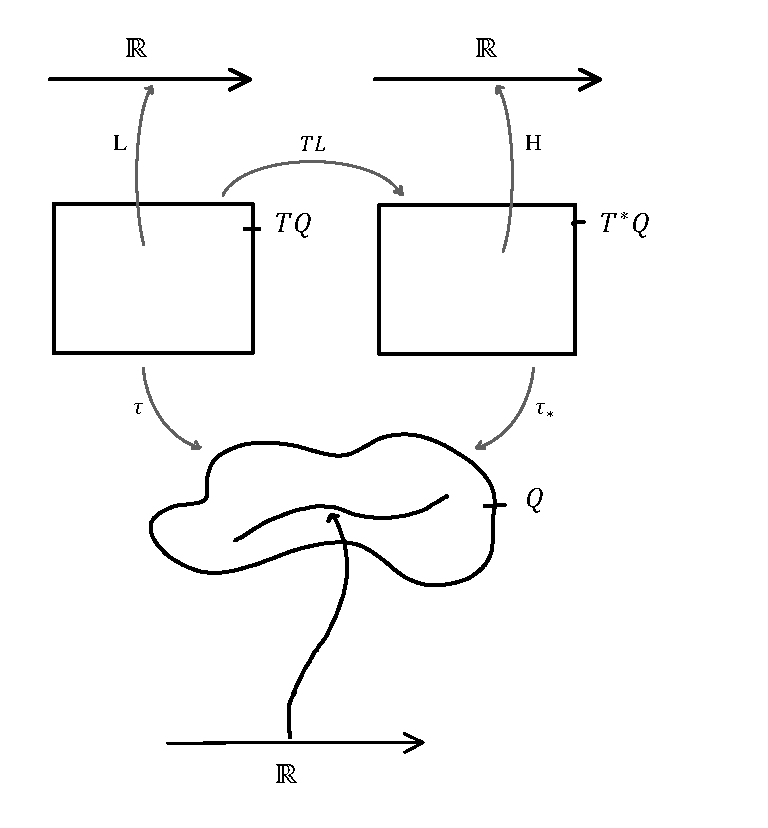
\includegraphics[width=\textwidth]{Presentazione/GeoMecFrameA} 
    				\end{block}
    			\end{column}
  			\end{columns}	
		\end{frame}
		
		\begin{frame}
			\frametitle{Formalismo Canonico Covariante}
  			\begin{columns}[T]
    			\begin{column}{.5\textwidth}
     				\begin{block}{Your textblock}
						% Your text here
						Passaggio Canonico Ordinario a Canonico Covariante (a finiti gradi)
						\\
						Parlare di Conf Sol e S
    				\end{block}
    			\end{column}
    		   	\begin{column}{.5\textwidth}
			    	\begin{block}{Your image}
						% Your image included here
						\includegraphics<1> [width=\textwidth]{Presentazione/GeoMecFrameA} 
						\includegraphics<2> [width=\textwidth]{Presentazione/GeoMecFrameB} 
						\includegraphics<3>[width=\textwidth]{Presentazione/GeoMecFrameC} 
    				\end{block}
    			\end{column}
  			\end{columns}		
		\end{frame}
	
		\begin{frame}
			\frametitle{Formalismo Covariante esteso}
  			\begin{columns}[T]
    			\begin{column}{.5\textwidth}
     				\begin{block}{Your textblock}
						% Your text here
						Il formalismo covariante si estende facilmente a sistemi più generali! ad esempio  i campi intesi come sistemi fisici con un set continuo di gradi \\
						Passaggio Canonico Covariante a Finiti Gradi a Canonico Covarianti a gradi continuo \\
						Parlare di Conf Sol e S	per i campi, notare che la definizione della lagrangiana è più delicate
    				\end{block}
    			\end{column}
    		   	\begin{column}{.5\textwidth}
			    	\begin{block}{Your image}
						% Your image included here
						\includegraphics<1> [width=\textwidth]{Pictures/FieMecFrame} 
						\includegraphics<2> [width=\textwidth]{Pictures/AbstractFieldTheory} 
    				\end{block}
    			\end{column}
  			\end{columns}		


		\end{frame}
		
		\begin{frame}
			\frametitle{Recuperare il formalismo canonico non covariante}		
			(extra) Recupare il formalismo canonico non covariante anche per i campi costruendo il dato su una superficie di Cauchy (ricordare che al continuo ci sono controesempi che darboux non vale)
			\\
			Lo si fa per sistemi su spazitempi globalmenente iperbolici. in breve sono varietà molto generali in cui è possibile definire per bene i problemi di cauchy
		\end{frame}

		\begin{frame}
			\frametitle{A che punto siamo?}		
			Fin qui abbiamo degli spazi canditati ad essere lo spazio delle fasi.
			Ciò che manca è la loro dotazione di una forma simplettica o di un algebra di Poisson di osservabili.

		\end{frame}


%\/\/\/\/\/\/\/\/\/\/\/\/\/\/\/\/\/\/\/\/\/\/\/\/\/\/\/\/\/\/\/\/\/\/\/\/\/\/\/\/\/\/\/\/\/\/\/\/\/\/\/\/\/\/\/\/\/\/\/\/\/\/\/\/\/\/\/\/\/
%				Parte 2 : 	"L'algoritmo di Peierls"
%\/\/\/\/\/\/\/\/\/\/\/\/\/\/\/\/\/\/\/\/\/\/\/\/\/\/\/\/\/\/\/\/\/\/\/\/\/\/\/\/\/\/\/\/\/\/\/\/\/\/\/\/\/\/\/\/\/\/\/\/\/\/\/\/\/\/\/\/\/		
%	\part{	Costruzione della struttura simplettica nel caso dei campi classici}
	\section{Metodo di Peierls}
	\frame{\sectionpage}
	
	\begin{frame}
		\frametitle{Cappello sul Metodo di Peierls }
			\begin{itemize}
				\item semplificare: usare i grafici già fatti e considerare solo i campi scalari
			\end{itemize}
			His essential insight was to consider the advanced and retarded “effect of one quantity (A) on another (B).” Here, A and B are to
be functions on H. 

			The advanced  and retarded  effects of A on B are then defined by comparing the original system with a new system defined by the action $S_\epsilon = S + \epsilon A$ and the same space H of histories. 
			Under retarded (advanced) boundary conditions for which the solutions $\phi \in S$ and $\phi_\epsilon	\in S_\epsilon$ coincide to the past (future) of the support of A, the quantity $B_0 = B(\phi)$ computed using $\phi$ will in general differ from $B_\epsilon = B(\phi_\epsilon)$ computed using $\phi_\epsilon$.
			For small epsilon, the difference between these quantities defines the retarded (advanced) effect of A on B through:
which depends on the unperturbed solution $\phi$.
	\end{frame}
	
	\begin{frame}
		\frametitle{I passi del metodo di Peierls}
		The procedure can be summarized in a few steps:
		\begin{enumerate}
			\item Consider a \emph{disturbance} $\chi$ that is a time-compact Lagrangian density .
			\item Construct the \emph{perturbation of a solution under the action of $\chi$}.
			%\emph{perturbation of a solution under the disturbance}. (correzione CD
			\item Define the \emph{effect of the disturbance} on a second Lagrangian functional.
			\item Assemble the mutual effects of two different Lagrangian densities to give a \emph{brackets}.
		\end{enumerate}	
	\end{frame}
	
	
	\begin{frame}
		\frametitle{ Concetto chiave dell'algoritmo di peierls}
		  	\begin{columns}[T]
    			\begin{column}{.5\textwidth}
     				\begin{block}{Your textblock}
						% Your text here
							Sono le \emph{disturbance lagrangiane}
    				\end{block}
    			\end{column}
    		   	\begin{column}{.5\textwidth}
			    	\begin{block}{Your image}
						% Your image included here
							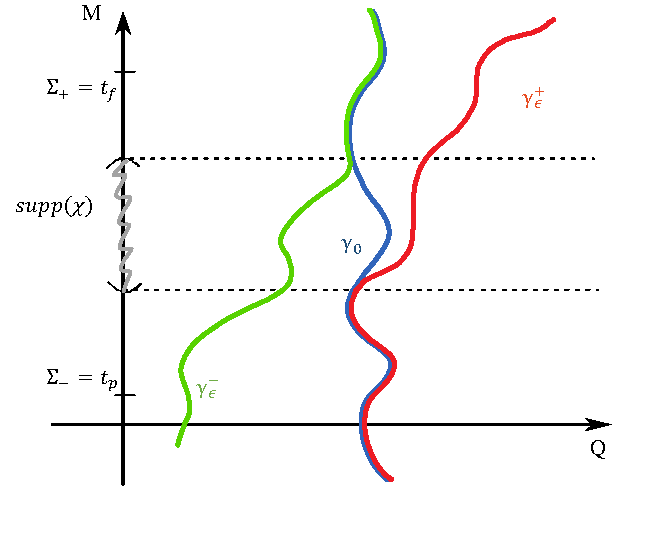
\includegraphics[width=0.5\textwidth]{Pictures/AdvRetSol}
    				\end{block}
    			\end{column}
    		\end{columns}
	\end{frame}
	
	
		\begin{frame}
		\frametitle{I Passi dell'algoritmo}
		  	\begin{columns}[T]
    			\begin{column}{.5\textwidth}
     				\begin{block}{Your textblock}
						\begin{itemize}
							\item
						\end{itemize}
    				\end{block}
    			\end{column}
    		   	\begin{column}{.5\textwidth}
			    	\begin{block}{Your image}
						% Your image included here
								\includegraphics<1>[width=\textwidth]{Pictures/GeometricPicture0}
								\includegraphics<2>[width=\textwidth]{Pictures/GeometricPicture1}
								\includegraphics<3>[width=\textwidth]{Pictures/GeometricPicture2}								
								\includegraphics<4>[width=\textwidth]{Pictures/GeometricPicture3}
								\includegraphics<5>[width=\textwidth]{Pictures/GeometricPictureLinear1}
								
    				\end{block}
    			\end{column}
    		\end{columns}
	\end{frame}
	
	\begin{frame}
		\frametitle{Dalle Parentesi di Peierls alla struttura di Poisson}
		  	\begin{columns}[T]
    			\begin{column}{.5\textwidth}
     				\begin{block}{Your textblock}
						\begin{itemize}
							\item
						\end{itemize}
    				\end{block}
    			\end{column}
    		   	\begin{column}{.5\textwidth}
			    	\begin{block}{Your image}
						\includegraphics<1>[width=\textwidth]{Pictures/compsupp_GeometricPicture0}
						\includegraphics<2>[width=\textwidth]{Pictures/compsupp_GeometricPicture1}
						\includegraphics<3>[width=\textwidth]{Pictures/compsupp_GeometricPicture2}
						\includegraphics<4>[width=\textwidth]{Pictures/compsupp_GeometricPictureLinear}
    				\end{block}
    			\end{column}
    		\end{columns}
	\end{frame}
	
	
	\begin{frame}
		\frametitle{Algebra di Poison realizzata tramite il metodo di Peierls}
		
	\end{frame}
	
	\begin{frame}
		\frametitle{Applicabilità del metodo di Peierls}	
			The Peierls' construction algorithm is well defined for a specific class of systems:
		\begin{enumerate}[A)]
			\item\label{HpPeierls1} Linear field theory: $E=(E,\pi,M;Q)$ is a vector bundle.
			%\item  Lagragian dynamics: $P=Q_\Lagrangian$ is a L.P.D.O.
			\item\label{HpPeierls2} $P=Q_\Lagrangian$ is a Green-hyperbolic linear partial differential operator.
			\item\label{HpPeierls3} $M$ is a globally hyperbolic spacetime.
			%\item Motion operator $P$ is a Green-hyperbolic.
		\end{enumerate}	
	\end{frame}
	
	\begin{frame}
		\frametitle{Peierls non è l'unica soluzione}
		Ci sono altri metodi provati essere equivalenti a peierls:
			Quello di wald sugli initial data e la sua versione covariante di Crnkovic riferita usualmente Covariant Phase space.
	
	\end{frame}
	
	
%\/\/\/\/\/\/\/\/\/\/\/\/\/\/\/\/\/\/\/\/\/\/\/\/\/\/\/\/\/\/\/\/\/\/\/\/\/\/\/\/\/\/\/\/\/\/\/\/\/\/\/\/\/\/\/\/\/\/\/\/\/\/\/\/\/\/\/\/\/
%				Parte 3 : 	"Realizzazione Specifica del campo di Jacobi"
%\/\/\/\/\/\/\/\/\/\/\/\/\/\/\/\/\/\/\/\/\/\/\/\/\/\/\/\/\/\/\/\/\/\/\/\/\/\/\/\/\/\/\/\/\/\/\/\/\/\/\/\/\/\/\/\/\/\/\/\/\/\/\/\/\/\/\/\/\/		
	%\part{Realizzazione per il Caso specifico dei campi di Jacobi}
	\section{Campo di Jacobi}
	\frame{\sectionpage}

	\begin{frame}
		\frametitle{ Ricordiamo il problema geodetico }
		  	\begin{columns}[T]
    			\begin{column}{.5\textwidth}
     				\begin{block}{Your textblock}
						\begin{itemize}
							\item<1-> Una varietà : una generalizzazione del piano cartesiano i.e. coordinatizzabile
							\item<2-> una Varietà (pseudo riemmaniana): è dotata di una metrica
							\item<3-> in presenza di una metrica posso formulare il problema geodetico
						\end{itemize}
    				\end{block}
    			\end{column}
    		   	\begin{column}{.5\textwidth}
			    	\begin{block}{Your image}
						\includegraphics<1>[width=\textwidth]{Presentazione/LocalChart}
						\only<1>{\footnote{credit \url{http://kahrstrom.com/}}}
						\includegraphics<2>[width=\textwidth]{Presentazione/Sfera}
						\only<2>{\footnote{Wip: esibire la presenza di una distanza (come lunghezza della curva di minima lunghezza?)}}
						\includegraphics<3>[width=\textwidth]{Presentazione/Sfera}
						\only<3>{\footnote{Wip: esibire il problema geodeca come circonferenze massimali}}
    				\end{block}
    			\end{column}
    		\end{columns}
	\end{frame}
	
	\begin{frame}
		\frametitle{I Campi di Jacobi}
		  	\begin{columns}[T]
    			\begin{column}{.5\textwidth}
     				\begin{block}{Your textblock}
						\begin{itemize}
							\item<1-> Tra tutti i campi lungo una fissata geodetica
							\item<2-> sono quelli che forniscono la variazione geodetica
							\item<3-> Catchword: campi di Jacobi come il moto di attrazione apparente di due gravi in caduta libera (fenomeno della deviazione geodetica)
						\end{itemize}
    				\end{block}
    			\end{column}
    		   	\begin{column}{.5\textwidth}
			    	\begin{block}{Your image}
						\includegraphics<1>[width=\textwidth]{Presentazione/Sfera}
						\only<1>{\footnote{Wip: Un campo tangente lungo un meridiano}}
						\includegraphics<2>[width=\textwidth]{Presentazione/Sfera}
						\only<2>{\footnote{Wip: animazione di una variazione Geodetica}}
						\includegraphics<3>[width=\textwidth]{Presentazione/Sfera}
						\only<3>{\footnote{Wip: Il campo di Jacobi è tangente alla variazione}}
    				\end{block}
    			\end{column}
    		\end{columns}
	\end{frame}

	\begin{frame}
		\frametitle{I Campi di Jacobi visti come un sistema fisico}
		  	\begin{columns}[T]
    			\begin{column}{.5\textwidth}
  						\begin{itemize}
							\item<1-> Il fibrato di Configurazione è..
							\item<2-> Le equazioni del moto sono ...
							\item<3-> Il metodo di Pierls è applicabile
						\end{itemize}
    			\end{column}
    		   	\begin{column}{.5\textwidth}
					bu
    			\end{column}
    		\end{columns}
	\end{frame}
	
	
	\begin{frame}
		\frametitle{Calcolo della formula di Peierls}
		  	\begin{columns}[T]
    			\begin{column}{.5\textwidth}
					bu
    			\end{column}
    		   	\begin{column}{.5\textwidth}
					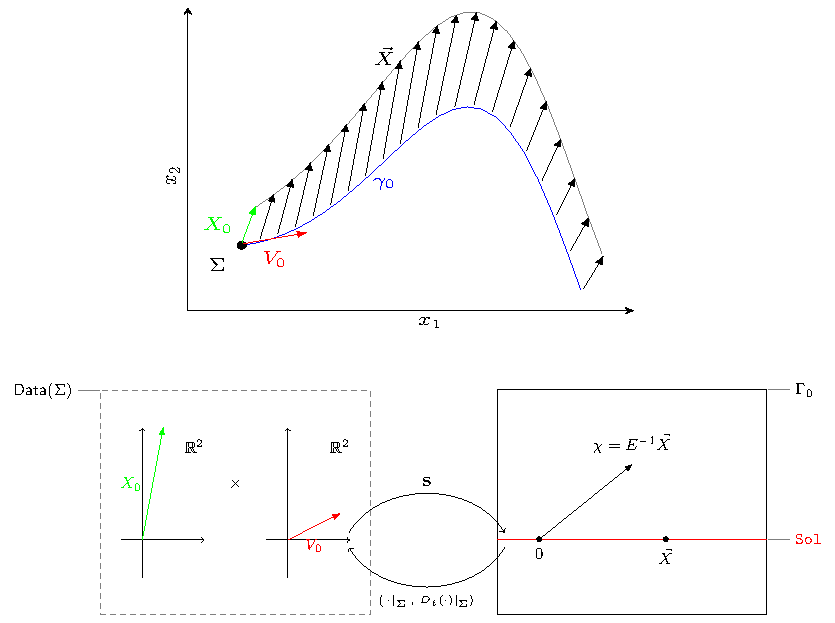
\includegraphics[width=\textwidth]{Pictures/Jacobi_GeometricPicturePanoramica}	
    			\end{column}
    		\end{columns}
	\end{frame}
	
	
	\begin{frame}
		\frametitle{Un esempio: I Campi di Jacobi su flat FRW}
		  	\begin{columns}[T]
    			\begin{column}{.5\textwidth}
					bu
    			\end{column}
    		   	\begin{column}{.5\textwidth}
					bu
    			\end{column}
    		\end{columns}
	\end{frame}	
	
	\begin{frame}
		\frametitle{Un altro esempio: Il campo di Jacobi 1D}
		  	\begin{columns}[T]
    			\begin{column}{.5\textwidth}
					bu
    			\end{column}
    		   	\begin{column}{.5\textwidth}
					\includegraphics<1>[width=\textwidth]{Pictures/Jacobi1D_GeometricPicture0}
					\includegraphics<2>[width=\textwidth]{Pictures/Jacobi1D_GeometricPicturePanoramica}	
    			\end{column}
    		\end{columns}
	\end{frame}	
	
	\begin{frame}
		\frametitle{ Qual'è l'interesse attorno al campo di Jacobi?}
					\begin{itemize}
				\item Abbiamo raccontato come si costruisce lo spazio simplettico per le teorie di campo secondi i due approcci alla Peierls e alla Wald.
				\item  Abbiamo provato che i due spazi simplettici sono isomorfi ma sono simplettomorfi solo in alcuni casi particolari.
				\item entrambe le due costruzioni sono esoteriche e calate dall'alto. 
					Mediamente vengono utilizzate come "black box" come ricette per dare una forma simplettica utile ma:
						\begin{itemize}
							\item a priori non c'è nessun motivo per cui le forme simplettiche che forniscono siano quelle "giuste".
							\item I singoli passaggi della costruzione non hanno giustificazione fisica.
							\item 	In breve: sappiamo il come, sappiamo che funziona ma non sappiamo "perchè".
						\end{itemize}
		\end{itemize}
	\end{frame}

	\begin{frame}
		\frametitle{ Qual'è l'interesse attorno al campo di Jacobi?}
					 Perchè Jacobi è un esempio pregnante
		\begin{itemize}
				\item
					In questo caso la costruzione di Wald non è ambigua. Data è isomorfo a $\Real^(2n)$ e la forma $\Sigma$ che viene imposta dalla procedura di wald corrisponde all'unica scelta possibile prevista dal teorema di Darboux (notare che anche per il semplice campo scalare lo spazio data è costituto da coppie di funzioni $C_0$ tutt'altro che finito dimensionale.
				\item l'interpretazione che cerchiamo è quasi di stampo "filosofico". Perchè la costruzione convoluta di peierls che parte dal considerare i disturbi lagrangiani è equivalente proprio all'unica forma simplettica su $Data=\Real^{2n}$ che praticamente coincide con lo spazio delle fasi classico?
				il problema sfuggente è "discutere sul perchè la costruzione di Peierls fornisce proprio la giusta usuale forma simplettica (parentesi $\Omega$) sullo spazio delle fasi classico?"\\
					( che su $\Real^{2n} $ sono univocamente fornite dal teorema di Darboux)			
		\end{itemize}
	\end{frame}

%\/\/\/\/\/\/\/\/\/\/\/\/\/\/\/\/\/\/\/\/\/\/\/\/\/\/\/\/\/\/\/\/\/\/\/\/\/\/\/\/\/\/\/\/\/\/\/\/\/\/\/\/\/\/\/\/\/\/\/\/\/\/\/\/\/\/\/\/\/
%				Fine	!!!
%\/\/\/\/\/\/\/\/\/\/\/\/\/\/\/\/\/\/\/\/\/\/\/\/\/\/\/\/\/\/\/\/\/\/\/\/\/\/\/\/\/\/\/\/\/\/\/\/\/\/\/\/\/\/\/\/\/\/\/\/\/\/\/\/\/\/\/\/\/		
\section*{Conclusioni}

	\begin{frame}
		\frametitle{ Conclusioni }
			\begin{itemize}
				\item cosa abbiamo capito dal caso di Jacobi?
				\item Interpretazione geometrica: punto chiave: ci sono 2 spazi la cui geometria soggiace al discorso: spazio delle soluzioni e spazio delle lagrangiane
			\end{itemize}
	\end{frame}
	
\end{document}